\documentclass[class=report, crop=false]{standalone}
\usepackage[subpreambles=true]{standalone}
\usepackage{import}

\begin{document}
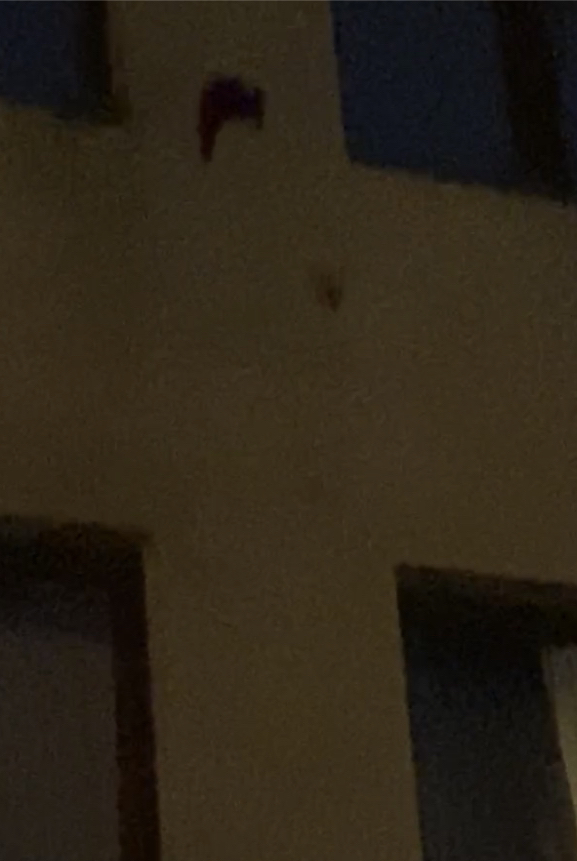
\includegraphics[width=\textwidth]{ext/parachutetest.png}
\captionof{figure}{The picture of the parachute being tested}
\newpage
The parachute tests were carried out from a rooftop of a large apartment building. \\
Assuming each floor is $3$ meters tall, we dropped the CanSat from 35 meters. \\
By analyzing the recording frame by frame, we calculated the CanSat was descending at $9\frac{\text{m}}{\text{s}}$. \\
As such, we have descided to use a different design of the parachute, unless we manage to change the current in such a way so as to allow us slower descend.
\end{document}
